%!TEX program=luatex

\newpage
\section{Introduction}
La réalisation d'un logiciel ou d'un système informatique doit être obligatoirement précédée d'une étape d'analyse et de conception qui a pour objectif de définir et de formaliser les étapes nécessaires du développement de l'application afin de rendre cette dernière plus fidèle aux besoins.

La première motivation de ce travail été de fournir un outil qui permet à l'utilisateur de faire ça revue de presse quotidienne de la façon la plus efficace et la plus enrichissante possible tout en considérant ses centres d'intérêts et préférences. 

Le logiciel que nous proposons enchaîne les processus de catégorisation, de résumé, de traduction et de recommandation d'articles de presse. Pour parvenir à réaliser cet ensemble de tâches en deux langues (Anglais et Arabe), nous allons présenter dans cette partie notre conception qui décrit d'une manière claire et précise le fonctionnement de chaque module du système. 


\section{Module de recommandation}
Dans cette partie, nous allons voir la conception détaillée de notre système de recommandation. Ci-dessous, nous présentons les deux approches proposées, la recommandation personnalisée et non personnalisée d'articles de presse.
    \subsection{Recommandation personnalisée\label{personal}}
    La recommandation d'articles est basée sur le contenu des profils utilisateurs. En effet, le profilage utilisateur débute lorsque l'utilisateur s'authentifie pour la première fois et à chaque fois les informations relatives à ses préférences sont récoltées et traitées.

    Cette étape nécessite le profilage de l'utilisateur et le calcul de similarité entre utilisateurs. Dans ce qui suit les détails de chacun.

        \subsubsection{Profilage d'un utilisateur}
        Elle consiste à déterminer les centres d'intérêts d'un utilisateur tout en se basant sur les articles lus par ce dernier. Pour cela, nous avons décidé d'utiliser une méthode de calcul des préférences afin de mieux cibler les utilisateurs et garantir une solution conforme aux caractéristiques de la recommandation pour les articles de presse. 

        Pour le calcul des préférences utilisateurs, nous avons utiliser une méthode de calcul qui permet à la fois de résoudre le problèmes de la récence \autoref{} et le démarrage à froid \autoref{}. Cette méthode testée s'avère très efficace par rapport aux méthodes existantes et décrites dans \autoref{}.

        Le calcul de la probabilité de sélection d'une catégorie pour un utilisateur est basé sur ses interactions avec les articles de presse disponible. Dés qu'un article est sélectionné, l'information est sauvegardée et utilisée pour la mise à jour du vecteur des probabilités de sélection des catégories préférées \autoref{}.

        L'exemple suivant présente un vecteur de probabilité de sélection pour les catégories préférées d'un utilisateur U :
            \[P(U) = {'sport': 0.7178, 'news': 0.1581, 'sci\_tech': 0.1492}\]            
        Il faut noter que la taille du vecteur de probabilité de sélection des catégories préférées est différentes d'un utilisateur à un autre.

        Ce vecteur se met à jour, comme déjà cité, après chaque interaction de l'utilisateur U avec l'article A de la catégorie C. Au fur et à mesure, la probabilité de sélection d'une catégorie C\textsubscript{i} augmente si cette dernière est sélectionnée, sinon, elle diminue pour donner moins d'importances aux articles qui font partie de cette catégorie.

        Ci-après les formules dédiées à la mise à jour des probabilités de sélection des catégories préférées :\\
            \[
            P(U, C) =
            \begin{cases}
                (1-{\alpha}) * {P(U, C)} + {\alpha} & \text{si } \text{article A est sélectionne} \\
                (1-{\alpha}) * {P(U, C)} & \text{sinon.}
            \end{cases}
            \]

        Avec initialement :\\
        \[
        \begin{cases}
            P(U, C) = 1 / \text{NbC } \forall \text{ C} \in \{categorie\textsubscript{1}, categorie\textsubscript{2}, ..., categorie\textsubscript{NbC}\}\\
            NbC : \text{nombre de categories}\\
            \alpha = \text{une constante empirique représentant le biais de la diminution}
        \end{cases}
        \]
        \begin{algorithm2e}[H]
        \SetAlgoLined
        \SetKwInOut{Input}{input}
        \SetKwInOut{Output}{output}
        \Input{A: Article, U: Utilisateur}
        \textbf{const :} \alpha = 0.1, NbC = nombre de catégories\\
        préférences = U.préférences\\
        catégorie = A.catégorie\\
        \eIf{catégorie \in préférences}{
            préférences[catégorie] = (1-{\alpha}) * {préférences[catégorie]} + {\alpha}\\
            \While{i < taille(préférences)}{
                \If{préférences[i] != catégorie}{
                    préférences[i] = (1-{\alpha}) * {préférences[catégorie]}\\
                }
            } 
        }
        {
            préférences[catégorie] = 1 / NbC
        }
        \caption{Algorithme de profilage d'un utilisateur}
        \end{algorithm2e}
        \subsubsection{Similarité entre utilisateurs}
        Afin de diversifier la recommandation des articles de presse, nous avons mis en place une méthode de calcul de similarité qui permet de recommander des articles par rapport à la similarité entre utilisateurs. 

        Selon \cite{euclidepreuve} qui propose une étude détaillée sur les mesures de similarité pour le filtrage collaboratif, il en est ressorti comme conclusion que la distance euclidienne était la mesure la plus adéquate en terme de précision et temps d'exécution. La formule de calcul de la distance euclidienne entre les préférences des utilisateurs est la suivante :

        \begin{itemize}[label={}, leftmargin=0cm]
            \item Soient U\textsubscript{1} et U\textsubscript{2} deux utilisateurs,
            \item P(U\textsubscript{1}) et P(U\textsubscript{2}) les vecteurs de probabilité de sélection des catégories préférées des deux utilisateurs respectivement,
            \item NbC\textsubscript{1} et NbC\textsubscript{2} le nombre de catégories préférées de chaque utilisateur,\  
            \item \[Sim({P(U\textsubscript{1})}, {P(U\textsubscript{2})}) = d({P(U\textsubscript{1})}, {P(U\textsubscript{2})}) = {\sqrt {\sum _{i=1, j=1}^{NbC\textsubscript{1},NbC\textsubscript{2}}(P(U\textsubscript{1}, C\textsubscript{i})-P(U\textsubscript{2}, C\textsubscript{j}))^{2}}}\]
        \end{itemize}

        Dans ce qui suit, un exemple de calcul de similarité entre deux utilisateurs :
        \[
        \begin{cases}
            P(U\textsubscript{1}) = {'sport': 0.7581, 'sci\_tech': 0.4492, 'religion': 0.3878, 'algeria': 0.0178,}\\
            P(U\textsubscript{2}) = {'religion': 0.8813,'sport': 0.4421, 'business': 0.3519}\\
        \end{cases}
        \]
        On ignore les probabilités de séléction des catégories non commune entre les deux utilisateurs.
        \[
        \begin{cases}
        d({'sport'}) = P(U\textsubscript{1},'sport')-P(U\textsubscript{2},'sport') = 0.7581 - 0.4421 = 0.32\\
        d({'religion'}) = P(U\textsubscript{1},'religion')-P(U\textsubscript{2},'religion') = 0.3878 - 0.8813 = −0,49 \\
        Sim({P(U\textsubscript{1})}, {P(U\textsubscript{2})}) = {\sqrt {d({'sport'})^{2}+d({'religion'})^{2}}}= {\sqrt{(0.32)^{2} + (-0.49)^{2}}} = 0,59
        \end{cases}
        \]
        \begin{algorithm2e}[H]
        \SetAlgoLined
        \SetKwInOut{Input}{input}
        \SetKwInOut{Output}{output}
        \Input{A: Article, U: utilisateur}
        \textbf{const :} seuil = 0.1\\
        utilisateurs = lire(base de profils)\\
        \While{i < taille(utilisateurs)}{
            \If{utilisateurs[i] != U}{
                sim = distance\_euclidienne(U.préférences, utilisateurs[i].préférences)\\
                \If{sim >= seuil}{
                    U.préférences += utilisateurs[i].préférences
                }
            }
        } 
        \caption{Algorithme de calcul de similarité entre utilisateurs}
        \end{algorithm2e}

    \subsection{Recommandation non personnalisée}
    La recommandation non personnalisée vise à recommander des articles pour des utilisateurs qui n'ont pas de comptes (i.e : qui sont non authentifiés), pour cela notre système effectue une recommandation selon le choix de lecture de l'utilisateur, c'est à dire par calcul de similarité entre l'article qui est entrain d'être lu et les nouveaux articles disponible. 

    Un pré-traitement est effectué sur chaque article comprend la suppression des mots vides et l'extraction des racines de mots. Ensuite, le sac à mots (Bag of Words) de l'article est converti en TF-IDF. La martice résultante de la conversion en TF-IDF est utilisée pour le calcul de la similarité de cosinus et les cinq articles les plus similaires seront recommandés. Le calcul de la similarité entre les articles est présenté ci-dessous :

    \begin{itemize}[label={}, leftmargin=0cm]
        \item Soient U un utilisateur, A\textsubscript{1} et A\textsubscript{2} deux articles de presse,
        \item A\textsubscript{1} a été déjà sélectionné et A\textsubscript{2} est un nouvel article,
        \item BoW(A\textsubscript{1}) et BoW(A\textsubscript{2}) les sacs à mots de chaque article,\\

        \item BoW(A\textsubscript{1}) = \{\begin{arab}'لواء', 'شفيق', 'مدير', 'مكتب', 'رئيس', 'مخلوع', 'مبارك', 'أراد', 'دائم', 'إيقاع', 'عمر', 'سليمان', 'مشير', 'طنطاوي', 'وصف', 'لواء', 'شفيق', 'عاش', 'قصر', 'رئيس', 'مصري', 'مخلوع', 'وفاة', 'عمر', 'سليمان', 'رئيس', 'مخابرة', 'مصري', 'نائب', 'مبارك', 'خسارة', 'أكبر', 'مصر', 'رجل', 'أفضل', 'رجل', 'شجع', 'صعب', 'تعويض', 'تحدث', 'لواء', 'شفيق', 'تصريح', 'علاقة', 'عمر', 'سليمان', 'رئيس', 'مخلوع', 'مبارك'\end{arab}\},

        \item BoW(A\textsubscript{2}) = \{\begin{arab}'استمر' 'نزاع', 'رئيس', 'وزير', 'نوري', 'مالكي', 'شيعي', 'خصم', 'حكم', 'أنصار', 'قائمة', 'عراقي', 'لواء', 'خلفية', 'اتهام', 'مالكي', 'نائب', 'رئيس', 'طارق', 'هاشمي', 'شجع', 'ضلع', 'عملية', 'إرهابي', 'أمر', 'أدى', 'تجميد', 'نشاط', 'حكومة', 'انسحاب', 'وزير', 'قائمة', 'عراقي', 'تفاقم', 'خلاف', 'نظر', 'مطالبة', 'تيار', 'رجل', 'صدري', 'قائمة', 'عراقي', 'علاقة', 'حل', 'برلمان'\end{arab}\},


        \item TF-IDF(A\textsubscript{1}) = \{0.0766346 , 0.05452615 , 0.4598076 , 0.1090523,  0.076346, 0.0766346, 0.0766346, 0.1090523, 0.16357845, ...\},

        \item TF-IDF(A\textsubscript{2}) = \{0.0261347 , 0.156338 , 0.229038 , 0.0730857,  0.0520013, 0.0816399, 0.0261347, 0.2299038, 0.16357845, ...\},

        \item \[sim\_cos(TF-IDF(A\textsubscript{1}), TF-IDF(A\textsubscript{2})) = \frac {TF-IDF(A\textsubscript{1}) \cdot TF-IDF(A\textsubscript{2})}{||TF-IDF(A\textsubscript{1})|| \cdot ||TF-IDF(A\textsubscript{2})||}\]
    \end{itemize}
    \begin{algorithm2e}[H]
        \SetAlgoLined
        \SetKwInOut{Input}{input}
        \SetKwInOut{Output}{output}
        \Input{A: Article, U: utilisateur}
        \Output{ListeArticlesSimilaires: Article}
        articles = lire(base de articles)\\
        \While{i < taille(articles)}{
            segmentation(articles[i])\\
            suppression\_mots\_vides(articles[i])\\
            racinisation(articles[i])\\
        }
        tf-idf = TF-IDF(articles)\\
        mat\_similarité = TRI(cosinus\_similarité(tf-idf))\\
        ListeArticlesSimilaires = mat\_similarité.articles\\
        \Return ListeArticlesSimilaires[:5]
        \caption{Algorithme de calcul de similarité entre articles}
    \end{algorithm2e}
% Deux types de recommandations d'articles de presse ont étaient présentées dans la section précédente qui dépendent du mode d'utilisation. L'algorithme \autoref{algo-recom} résume le fonctionnement des deux types de recommandation.\\\\ 
%     \begin{algorithm2e}[H]\label{algo-recom}
%         \SetAlgoLined
%         \SetKwInOut{Input}{input}
%         \SetKwInOut{Output}{output}
%         \Input{A: Article, U: utilisateur}
%         \Output{ListeArticlesSimilaires: Article}
%         % \eIf{U est authentifié}{
%         % }
%         \caption{Algorithme de calcul de similarité entre articles}
%     \end{algorithm2e}
%%~~~~~~~~~~~~~~~~~~~~~~~~~~~~~~~~~~~~~~~~~~~~~~~~~~~~~~~~~~~~~~~~~~~~~~~~~~~~~~~~~~~~~~~~~~~~~~~~~%%

\section{Module de catégorisation d'article de presse}
Le premier module sur lequel nous avons travailler, c'est la catégorisation d'articles de presse. Nous avons expérimenter plusieurs techniques proposées dans la littérature. Nous présentons ci-après chaque approche, ses résultats, ses points forts et ses faiblesses.

En se basant sur les travaux de \cite{categorisation} pour l'Anglais et \cite{categorisation} pour l'Arabe, nous avons entraîné nos modèles sur des corpus d'articles de différentes sources afin de garantir la diversité dans nos données (plus de détails dans le chapitre 4\ref{chapter4}).
À REVOIR!!

    \subsection{Approches expérimentées\label{approches}}
    Toutes les approches utilisées sont basées sur l'apprentissage automatique, supervisé et non supervisé. 
     
     \subsubsection{Organisation des données}
      Apprentissage non supervisé :
     
     
     
       Apprentissage supervisé:
     
      À la fin de la phase de pré-traitement, nous avons définie une structure pour faciliter l'exploration des datasets. Ci-dessous la structure choisie :
     \begin{itemize}
        \item{\textbf{id} :}un identifiant unique de l'article,
        \item{\textbf{contenu} :}les différents paragraphes de l'article,
        \item{\textbf{catégorie} :}la catégorie de l'article extraite depuis la source.
     \end{itemize}
      
        \subsection{Processus de catégorisation}
         
            \subsubsection{Pré-traitement des articles de presse}
           
             Plusieurs opérations de pré-traitements ont été effectuées. Ci-après les étapes suivies :
            \begin{enumerate}
                \item{\textbf{Segmentation (Tokenization) et suppression des mots vides :} }permet d'extraire toutes les entités lexicales d'un article donné. La segmentation est suivie de la suppression des tokens non utiles tel que la ponctuation, les pronoms, les déterminants, etc.\\ 
                          
                % Exemple :
                %          بلغ مستوى التضخم 4.3 بالمائة إلى غاية أفريل 2018، بعد أن  كان في حدود 4.6 بالمائة شهر مارس الماضي.
                
                % Aprés segmentation : on aura une liste de mots.
                                       
                %                        ['بلغ', 'مستوى', 'التضخم', '4.3', 'بالمائة','إلى','غاية','أفريل', '2018', '،','بعد', 'أن', 'كان', 'في', 'حدود',' 4.6 ', 'بالمائة', 'شهر', 'مارس', 'الماضي','.']
                                                          
                % Liste des mots vides de la phrase précédente.                                         
                
                                                               
                %                                        ['بعد', 'أن', 'كان', 'في', 'ب','إلى','.','4.3','2018', '،','4.6']  
                
                % Aprés suppression des mots vides :
                
                
                %                           ['بلغ', 'مستوى', 'التضخم','المائة','غاية','حدود','المائة', 'شهر', 'مارس', 'الماضي']  
                
                
                % \item{\textbf{Racinisation (Stemming) :} }les mots d'un document sont représentés par leurs racines plutôt que par les mots d'origine. Plusieurs variantes d'un terme peuvent ainsi être groupées dans une seule forme représentative, ce qui réduit le nombre des termes distincts nécessaires pour représenter un document.\\
                
                % Exemple :
                
                
                %                                ['بلغ', 'مستوى', 'التضخم','المائة','غاية','حدود','المائة', 'شهر', 'مارس', 'الماضي']  
               
                
                
                % \item{\textbf{N-grammes :} }les N-grammes permettent de construire une sous-séquence de n mots consécutives. Ils permettent de contextualiser l'ordre d'apparition d'un ensemble de mots.\\
                
                % Exemple : 
                %          بلغ مستوى التضخم 4.3 بالمائة إلى غاية أفريل 2018، بعد أن  كان في حدود 4.6 بالمائة شهر مارس الماضي.      
                
                
                \item{\textbf{Extraction des caractéristiques :} }avec l'utilisation de TF-IDF, le sac de mots représentant un article sera convertit en valeurs numériques décrivant la fréquence d'occurrence de chaque mot par rapport à l'ensemble des articles du corpus et à l'article lui même.\\
            
        
            \end{enumerate}

        \subsubsection{Basées sur l'Apprentissage Non Supervisé}
        
        \begin{itemize}
            \item{LDA (Latent Dirichlet Allocation) : }
            Latent Dirichlet Allocation (LDA) est un modèle probabiliste génératif qui permet de décrire des collections de documents de texte ou d’autres types de données discrètes. LDA fait partie d’une catégorie de modèles appelés “topic models”, qui cherchent à découvrir des structures thématiques cachées dans des vastes archives de documents. Ceci permet d’obtenir des méthodes efficaces pour le traitement et l’organisation des documents de ces archives: organisation automatique des documents par sujet.
            
        \end{itemize}
        
        \subsubsection{Basées sur l'Apprentissage Supervisé}
        \begin{itemize}
            \item{Naïve de Bayes : }
            c'est une méthode connue de l'Apprentissage automatique supervisé. Un de ses avantages en plus d'être un modèle simple, c'est qu'ils renvoient non seulement la prédiction mais aussi le degré de certitude, ce qui peut être très utile dans certaines applications. Mais en ayant un problème à classes multiples, cette approche nous a donnés des résultats très modeste en un temps d'exécution assez importants, ce qui nous a poussé à abandonner son utilisation.\\
            
            \item{Arbres de décision : }
            peuvent être assistés par un expert. Ces principaux avantages sont : robuste face aux données aberrantes, pas très sensible aux données manquantes, possibilité d’intervenir dans la construction de l’arbre, etc. Son principale inconvénient reste la dépendance très forte entre la taille de la base d’apprentissage et les performances.\\
            
            \item{SVM (Support Vector Machines) : }
            NOT YET
            
            
            \item{Descente de Gradient Stochastique : }
            NOT YET
        \end{itemize}

%%~~~~~~~~~~~~~~~~~~~~~~~~~~~~~~~~~~~~~~~~~~~~~~~~~~~~~~~~~~~~~~~~~~~~~~~~~~~~~~~~~~~~~~~~~~~~~~~~~%%

\section{Module de résumé automatique}
Pour ce module de résumé automatique, nous avons choisi un résumeur automatique extractif \cite{notreresume} basé sur les plongements de mots (Word embeddings)!!!!!!! comme décrit dans le chapitre précédent \autoref{}.
Ci-dessous la présentation des différentes approches expérimentées.
    \subsection{Résumé extractif par Apprentissage Supervisé}
    Nous avons, tout d'abord, expérimenté l'approche proposé dans \ref{riad-belkbir} qui est basée sur un apprentissage automatique supervisé en utilisant un dataset annoté manuellement. 
        \subsubsection{Corpus et datasets}
        Le dataset contient plus de 70 articles. Il est dédié principalement au résumé automatique par apprentissage supervisé pour la langue Arabe, mais peut être utilisé également dans d'autres applications, telles que la compression des textes.

        L'annotation consiste en l'attribution de quatre type d’étiquettes possibles à chaque phrase de l'article :
            \begin{itemize}
                \item S (select) : phrase importante, à prendre en considération dans la construction du résumé.
                \item R (remove) : cette phrase est à supprimer, son absence n'affecte pas le sens du résumé.
                \item F (fusion) : fusion de deux phrases (ou plus).
                \item C (compress) : compression d'une phrase on supprimant les synonymes et les redondances dans le sens.\\
            \end{itemize}

        \subsubsection{Pré-traitement et structure du dataset}
        Tout les articles du dataset sont sous le format XML, chaque article a son propre identifiant et divisé en paquets de phrases selon l'opération effectuée. Ci-après la figure \ref{xml-structure} qui montre un exemple du dataset : 
        \begin{figure}[H]
            \centering
            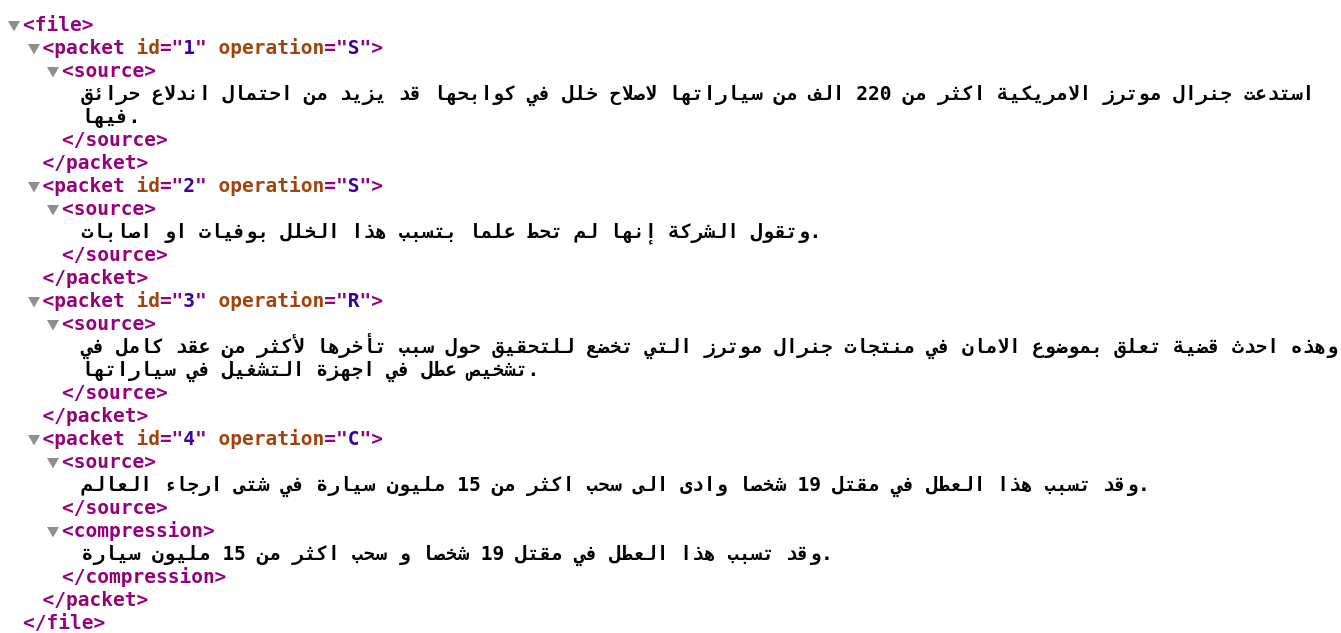
\includegraphics[height=220pt,width=430pt]{img/chapter4/xml.png}
            \caption{Structure d'un article du dataset}
            \label{xml-structure}
        \end{figure}
        L'approche basée sur l'apprentissage automatique demandait un très grand nombre d'articles résumés, ce qui nous a poussé à l'abandonner.

    \subsection{Résumé extractif par Machine de Boltzman}
    L'approche proposée dans \cite{boltzman} utilise un modèle d'apprentissage profond afin de prédire les phrases les plus importantes dans un texte donnée en utilisant 9 caractéristiques sur chaque phrase. Elle consiste en trois grande phases: l'extraction des caractéristiques, la conversion en valeurs numériques et la génération du résumé à partir des scores de chaque phrase. 

    Les caractéristiques extraites sont les suivantes :
    \begin{enumerate}
        \item{Nombre de mots clés}
        \item{Position de la phrase dans le texte}
        \item{Longueur de la phrase}
        \item{Position de la phrase dans le paragraphe}
        \item{Nombre de noms propres}
        \item{Nombre d'entités numériques}
        \item{Nombre d'entités nommées}
        \item{TF-ISF (Term Frequency- Inverse Sentence Frequency)}
        \item{Similarité avec la phrase centroïde}
    \end{enumerate} 

    \subsection{Résumé automatique extractif par Plongement de mots\ref{plongement}}
    L'approche proposée par l'équipe de recherche du département informatique de l'Université de Bari en Italie \cite{bari}, est basée sur la similarité textuelle entre la phrase centroïde et les autres phrases du texte en utilisant les plongements de mots (Word embeddings)\ref{}. Le plongement de mots utilisé dans cette approche est un modéle skip-gram entrainé sur le contenu de Wikipédia \cite{} en utilisant la bibliothèque fasttext du laboratoire en intelligence artificielle de facebook qui ont dévellopé des modéles pour 294 langues différentes \cite{fasttext}. parmi les modéles developpé, nous allons nous intérésser a celui de l'anglais et l'arabe. La conception et l'algorithme de réalisation sont détaillés dans \ref{plongement}. Ci-dessous, nous allons présenter les étapes de conception du résumé automatique.

        \subsubsection{Prétraitement des articles}
        Dans cette phase, il suffit juste de segmenter le texte, le tokeniser et supprimer les mots vides. Ceci étant dû au fait que le plongement de mots que nous allons utiliser (le modèle Skip-Gram entraîné sur le contenu Wikipédia) servira entre autre a détecter les régularités linguistiques des  mots de la même racine. par exemple : le mot le plus similaire a "Algeria" est le mot "Algerian" \ref{}, c'est pour cela que le stemming n'est pas utilisé dans ce cas.

         \begin{algorithm2e}[H]
           \SetAlgoLined
          \SetKwInOut{Input}{input}
          \SetKwInOut{Output}{output}
          \Input{A: Article}
          \Output{Listesdestokens: token}
          
          Lire(A)\\
          C=Segmentationdesphrases(A)\\
          T=Tokenisation(C)\\
          Listedestokens=Suppression\_mots\_vides(T)\\
          
          \Return {Listesdestokens}
         \caption{Algorithme de prétraitment du résumé}
        \end{algorithm2e}

       \subsubsection{Construction d'un vecteur de centroïde}
        Après l'étape de prétraitement, place a la construction des vecteurs de centroïde. Afin de construire un vecteur centroïde en utilisant les plongement de mots, nous sélectionnons d'abord les mots significatifs dans le document. Pour cela, nous calculons le poids Tf-IDF de chaque mots de chaque document, ensuite nous sélectionnons les mots ayant le poids Tf-IDF supérieur à une constante empirique fixé au tout début de cette phase qui désignera un seuil de document (idf). Ainsi, nous calculons l'encastrement du centroïde comme la somme des mots les mieux classés dans le document en utilisant les plongements de mots de Wikipédia comme le montre l'equation suivante :

             \begin{equation*}
             C = \sum_{\substack{w\in D\\
                             tf-idf(w)>t }}
                    E[idx(w)]
             \end{equation*}
             
             C: l'encastrement centroïde lié au document D.
             et 
             idx(w) : une fonction qui retourne l'indice du mot dans le vocabulaire.
             
             exemple :
             
             \begin{figure}[H]
                \centering
                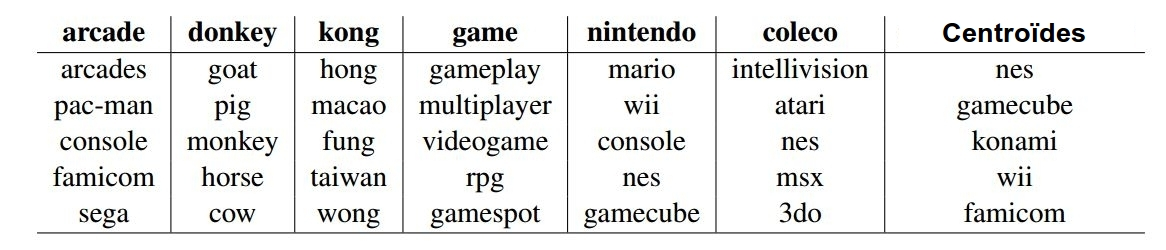
\includegraphics[height=120pt,width=380pt]{img/chapter3/centroideembed.jpg}
                \caption{Constuction des vecteurs centroïde}
                \label{Constuction des vecteurs centroïde}
             \end{figure}
             
%\begin{algorithm2e}[H]
%   \SetAlgoLined
%   \SetKwInOut{Input}{input}
%   \SetKwInOut{Output}{output}
%   \Input{S,Scores,st,limite}
%   \Output{Résumé}
    
%   S=Tri(phrases,Scores)\\
%   $k \gets 1$
    
%   \For{$i\gets1$ \KwTo $m$ }{
%       $longeur \gets Longeur(résumé)$
        
%       \If{longeur > limite}{
%           \Return résumé\\
%           $sv \gets somme_des_vecteurs(S[i])$\\
%           $inclus \gets vrai$\\}
%       \For{$j\gets1$ \KwTo $k$ }{
%           $SV2 \gets somme_des_vecteurs(résumé[i])$\\
%           $sim \gets Similarité(SV,SV2)$\\
%           \If{sim > st}{
%               $Inclus \gets FAUX$ \\}
%       }
%       \If{inclus}{
%           $résumé[k]\gets S[i]$\\
%           $k\gets k+1$\\      
%       }
%   }
%   \caption{Algorithme de construction d'un vecteur centroide}
%\end{algorithm2e}

         \subsubsection{Notation des phrases}
         Dans ce processus, pour chaque phrase du document on crée un plongement pour la phrase en additionnons les plongements de mots de chaque terme dans la phrase.

        \begin{equation*}
         S\textsubscript{j} = \sum_{\substack{w\in S\textsubscript{j}}}
         E[idx(w)]
        \end{equation*}

        Afin de calculer le score finale de la phrase, on calcule la similarité de cosinus entre le plongement de la phrase S\textsubscript{j} et le plongement de la phrase centroide C.
        
        \[sim\_cos(C,S\textsubscript{j}) = \frac {C \cdot S\textsubscript{j}}{||C|| \cdot ||S\textsubscript{j}||}\]
                    
                    \begin{figure}[H]
                        \centering
                        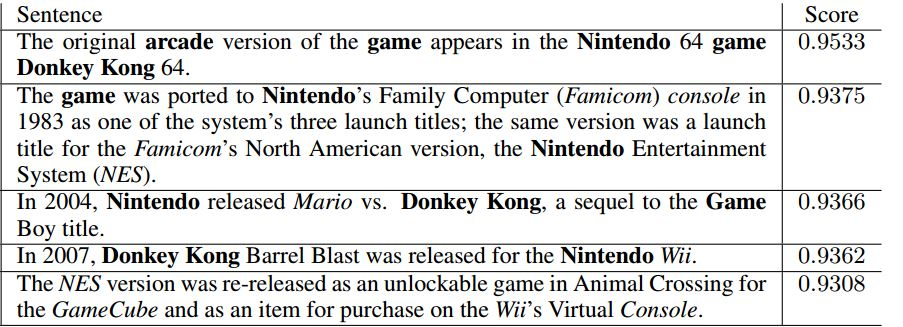
\includegraphics[height=150pt,width=380pt]{img/chapter3/scoreembed.jpg}
                        \caption{Notation des phrases}
                        \label{Notation des phrases}
                    \end{figure}

\subsubsection{Séléction des phrases}
Pour chaque phrase du document, on calcule la \emph{similarité de cosinus} entre elle et la phrase centroïde du document. Les phrases sont ensuite triées par ordre décroissant de leurs scores de similarité. Les phrases les mieux classées sont itérativement sélectionnés et ajoutés au résumé jusqu'à ce que la limite (taille du résumé) soit atteinte. Afin de satisfaire la propriété de redondance, au cours de chaque itération nous allons calculer la \emph{similarité de cosinus} entre la phrase a venir et chacune déjà dans le résumé.
Il est a noter qu' un seuil a été fixé afin de rejeter toutes les phrases qui ont une similarité très élevé par rapport a une phrase afin d'éviter cette redondance.

\begin{algorithm2e}[H]
    \SetAlgoLined
    \SetKwInOut{Input}{input}
    \SetKwInOut{Output}{output}
    \Input{S,Scores,st,limite}
    \Output{Résumé}
    
    S=Tri(phrases,Scores)\\
    $k \gets 1$
    
     \For{$i\gets1$ \KwTo $m$ }{
        $longeur \gets Longeur(résumé)$
        
        \If{longeur > limite}{
            \Return résumé\\
            $sv \gets somme_des_vecteurs(S[i])$\\
            $inclus \gets vrai$\\}
            \For{$j\gets1$ \KwTo $k$ }{
                $SV2 \gets somme_des_vecteurs(résumé[i])$\\
                $sim \gets Similarité(SV,SV2)$\\
                \If{sim > st}{
                    $Inclus \gets FAUX$ \\}
                }
        \If{inclus}{
            $résumé[k]\gets S[i]$\\
            $k\gets k+1$\\      
        }
     }
    \caption{Algorithme de Séléction des phrases}
\end{algorithm2e}

%%~~~~~~~~~~~~~~~~~~~~~~~~~~~~~~~~~~~~~~~~~~~~~~~~~~~~~~~~~~~~~~~~~~~~~~~~~~~~~~~~~~~~~~~~~%%

\section{Module de traduction}

Dans ce module, nous avons a la base choisi d'intégrer uniquement une solution de de traduction existante. Ci-dessous, une figure qui montre le processus de traduction automatique.


%ici image%%%%%%%%

Afin d'intégrer un bon système de traduction automatique, nous avons explorer 2 sources principales, la première était destiné a une utilisation professionnelle, de lus la version gratuite offrait une traduction pour des textes de taille limités. et la deuxième était la solution adaptée a notre système. Elle était a la fois accessible et offrait des possibilités de traduction pour des textes longs (Articles de presse, etc). 

\section{Conception de la base de données}
Le choix a été porté sur les bases de données NoSQL (\autoref{nosql}) vu la structure très dynamique des articles de presse mais aussi des profils utilisateurs.

MongoDB est une base de données orientée document écrite en C++ \cite{NOSQL3}. Les objets sont stockés en série sous la forme BSON.
Les objets n'ont pas besoin d'avoir la même structure ou les mêmes champs et les champs communs n'ont pas besoin d'avoir le même type, permettant ainsi un stockage de schéma flexible. À cet effet, nous présentons ci-dessous, sous ce format, la "collection d'articles" et la "collection des profils".

\subsection{Collection d'articles}
Les articles extraits depuis différentes sources sont tous sauvegardés sous une structure définie au préalable, prenant en considération les différences entre les formats suivies par les revu de presse. 

À cet effet nous avons choisi \emph{JSON} qui est un format léger d'échange de données. Il est facile à lire ou à écrire pour des humains\cite{json} et est pris en charge par tout les langages de programmation.

Chaque article est représenté comme suit:
\begin{itemize}
    \item \textbf{Identifiant, \textquotedbl \_id\textquotedbl: } identifiant unique d'un article de presse.
    \item \textbf{Langue, \textquotedbl language\textquotedbl:} la langue dans laquelle l'article est écrit.
    \item \textbf{Titre, \textquotedbl title\textquotedbl:} le titre de l'article.
    \item \textbf{Source, \textquotedbl source\textquotedbl:} nom de la revue de presse source.
    \item \textbf{Auteur, \textquotedbl author\textquotedbl:} on sauvegarde le nom de l'auteur.
    \item \textbf{Contenu, \textquotedbl content\textquotedbl:} contenu de l'article de presse.
    \item \textbf{Horaire, \textquotedbl publishedAt\textquotedbl:} date et heur local de publication.
    \item \textbf{Lien de l'article, \textquotedbl url\textquotedbl:} lien vers la page de l'article originale.
    \item \textbf{Lien de l'image, \textquotedbl urlToImage\textquotedbl:} lien vers l'image principale de l'article originale.
    \item \textbf{Catégorie, \textquotedbl categoryPredicted\textquotedbl:} catégorie de l'article inférée en utilisant nos modèles.
    \item \textbf{Résumé, \textquotedbl summaryGenerated\textquotedbl:} résumé automatique générée.
    \item \textbf{Traduction, \textquotedbl translatedContent\textquotedbl:} contenu de l'article de presse traduit.\\
\end{itemize}

Voici maintenant un exemple d'un document de la collection d'articles.
\begin{lstlisting}[style=code]
{
'_id': '5afc18571d41c833a8632a24', 
'language': 'en',
'title': "Smart's stellar Game 2 play draws Cavs praise", 
'source': 'espn', 
'author': 'Chris Forsberg', 
'content': 'LeBron James and Tyronn Lue explain what they think of Marcus...'
'publishedAt': '2018-05-16T05:48:55Z', 
'url': 'http://espn.go.com/nba/id/235168',
'urlToImage': 'http://espn.go.com/nba/id/235168/main.png',  
'categoryPredicted': 'sport', 
'summaryGenerated': 'The Celtics improved to 8-2 since Smart returned...', 
'translatedContent': '?????? ???? ???? ?? ???? ?? ?? ????? ?????? ????? ?? ??????? ????? ?????? ??? ????....', 
},
\end{lstlisting}

\subsection{Collection de profils}
Le profile d'utilisateur regroupe très peu d'informations dans le but de protéger la vie privée. Cependant, les catégories et les sources préférées par l'utilisateur sont sauvegardées. 

Un profil utilisateur est représenté comme suit :
\begin{itemize}
    \item \textbf{Identifiant, \textquotedbl  \_id\textquotedbl : } identifiant unique.
    \item \textbf{Nom d'utilisateur, \textquotedbl  username\textquotedbl : } nom d'utilisateur unique.
    \item \textbf{Mot de passe, \textquotedbl  password\textquotedbl : } mot de passe pour l'authentification crypté.
    \item \textbf{Adreese mail, \textquotedbl  email\textquotedbl : } email de l'utilisateur.
    \item \textbf{Catégories préférées, \textquotedbl  preferences\textquotedbl : } vecteurs de catégories préférées .
    \item \textbf{Sources préférées, \textquotedbl  sources\textquotedbl : } noms des sources de revues de presse préférées. 
\end{itemize}

Ci-dessous un exemple d'un document de la collection de profils :
\begin{lstlisting}[style=code]
{
'_id': '5afc18571d41c833a8632a24', 
'username': 'yankheloufi'
'password': 'CAESEMgZsfgjSKT7GvZNAtFJaAs'
'email': 'yk@usthb.dz',
'categories': {
'entertainment': '0.63',
'world': '0.42',
'health': '0.12',
},
'sources': [
'wello-mag', 'al-jazeera-english', 'bbc-news', 
],
},
\end{lstlisting}


%%%%%%%%%%%%%%%%%%%%%%%%%%%%%%%%%%%%%%%%%%%%%% Architecture globale %%%%%%%%%%%%%%%%%%%%%%%%%%%%%%%%%%%%%%%%%%%%%%%%%

\section{Architecture globale de "Feedny"}
Dans cette partie, nous allons présenter l'architecture globale de notre système, cette dernière est déployé sous la forme d'une architecture 3-tiers. Ci-dessous, nous présentons ce qu'est une architecture 3-tiers ainsi que son avantage avant d'expliciter un schéma de l'architecture globale.

\subsection{Présentation de l’architecture 3-tiers}
Une application Web possède souvent une architecture 3-tiers.
La couche DAO : " Data Access Object " s’occupe de l’accès aux données, le plus souvent des
données persistantes au sein d’un SGBD.

La couche métier : implémente les algorithmes " métier " de l’application. Cette couche est indé-
pendante de toute forme d’interface avec l’utilisateur.C’est généralement la couche la plus
stable de l’architecture. Elle ne change pas si on change l’interface utilisateur ou la façon
d’accéder aux données nécessaires au fonctionnement de l’application.

La couche interface utilisateur : interface (graphique souvent) qui permet à l’utilisateur de pi
loter l’application et d’en recevoir des informations.
FIGURE 3.1 – Architecture 3-tiers

\begin{figure}[H]
    \centering
    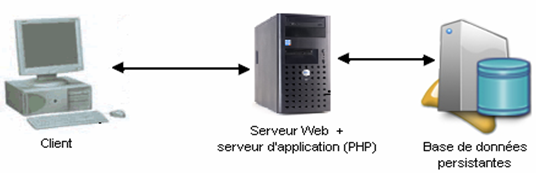
\includegraphics[height=100pt,width=400pt]{img/chapter3/tiers.png}
    \caption{Diagramme présentant les cas d'utilisations}
\end{figure}

\subsection{Avantage de l’architecture multi-tiers}
L’avantage principal d’une architecture 3-tiers (multi-tiers) est la facilité de déploiement.L’application
en elle même n’est déployée que sur la partie serveur.
Le client ne nécessite qu’une installation et une configuration minime.
En effet il suffit d’installer un navigateur web compatible avec l’application pour que le client
puisse accéder à l’application.
Cette facilité de déploiement aura pour conséquence non seulement de réduire le coût de déploie
ment mais aussi de permettre une évolution régulière du système. Cette évolution ne nécessitera
que la mise à jour de l’application sur le serveur applicatif.[4]

\subsection{Schéma fonctionnel de \textquotedbl Feedny\textquotedbl}
\begin{figure}[H]
    \centering
    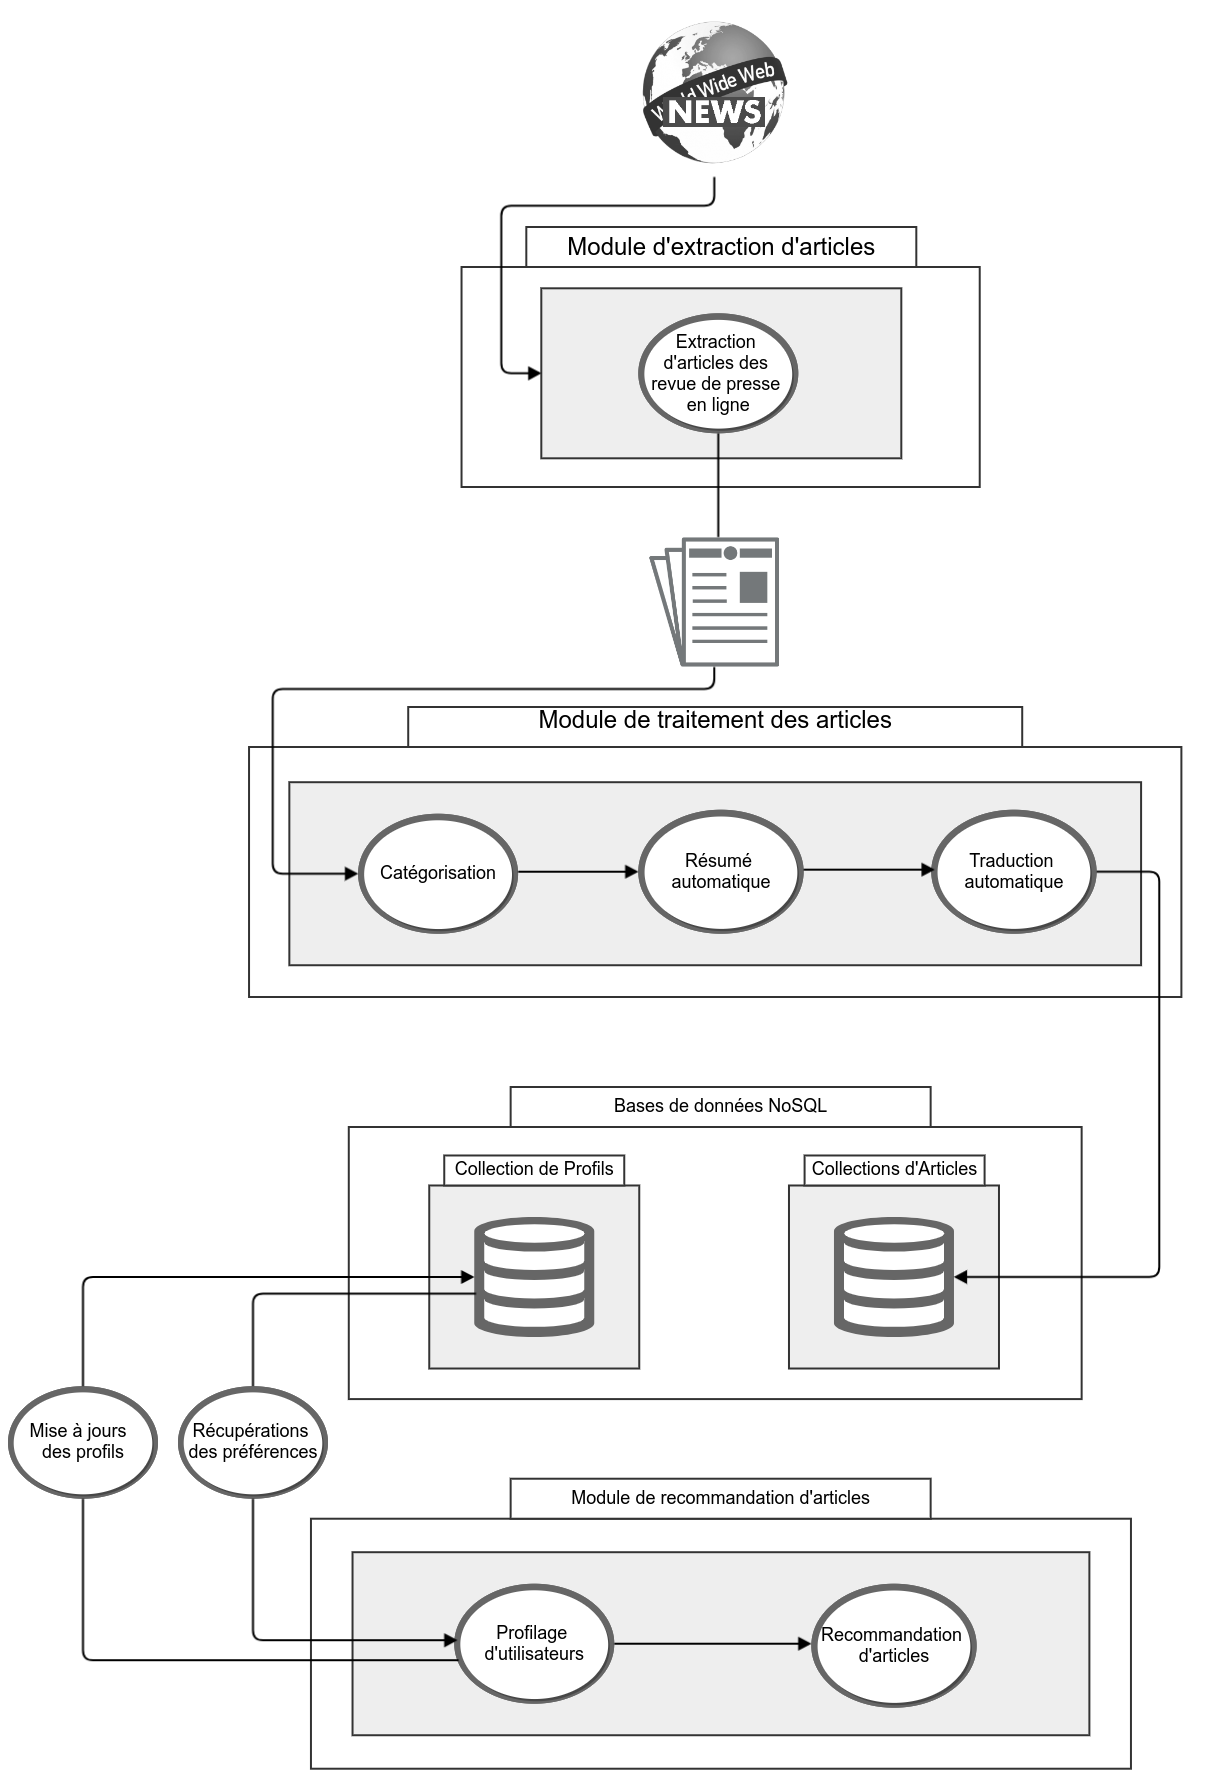
\includegraphics[height=600pt,width=450pt]{img/chapter3/global.png}
    \caption{Diagramme présentant les cas d'utilisations}
\end{figure}

%%%%%%%%%%%%%%%%%%%%%%%%%%%%%%%%%%%%%%%%%%%%%% Shéma %%%%%%%%%%%%%%%%%%%%%%%%%%%%%%%%%%%%%%%%%%%%%%%%%

\section{Schémas conceptuels de "Feedny"}
Nous allons présenter dans cette partie, la façon avec laquelle le logiciel fournit les différentes fonctionnalités. Celle-ci décrit d'une manière claire et précise, le fonctionnement du futur système en utilisant un langage de modélisation. 

Nous avons choisi la méthode UML (Unified Modeling Language), qui est une notation graphique conçue pour représenter, spécifier et construire les systèmes logiciels. UML utilise des techniques orientées objets pour la modélisation des systèmes, depuis la conception jusqu'à la maintenance, d'une manière compréhensible par l'homme et disposant de qualités formelles suffisantes pour être traduites automatiquement en code source.\cite{UML}

\subsection{Diagramme de cas d'utilisation}
"Le diagrammes de cas d'utilisation (initié par Ivar Jacobson en 1992 dans la méthode OOSE) est un type de diagramme UML qui permet de définir les besoins des acteurs dans un système quelconque en établissant les fonctionnalités attendues et en organisant les besoins. Il peut être aussi utilisés ensuite comme moyen d'organisation du développement du logiciel, notamment pour la structuration et le déroulement des tests du logiciel".\cite{UML}

\subsubsection{Diagramme de cas d'utilisation de "Feedny"}
\begin{figure}[H]
    \centering
    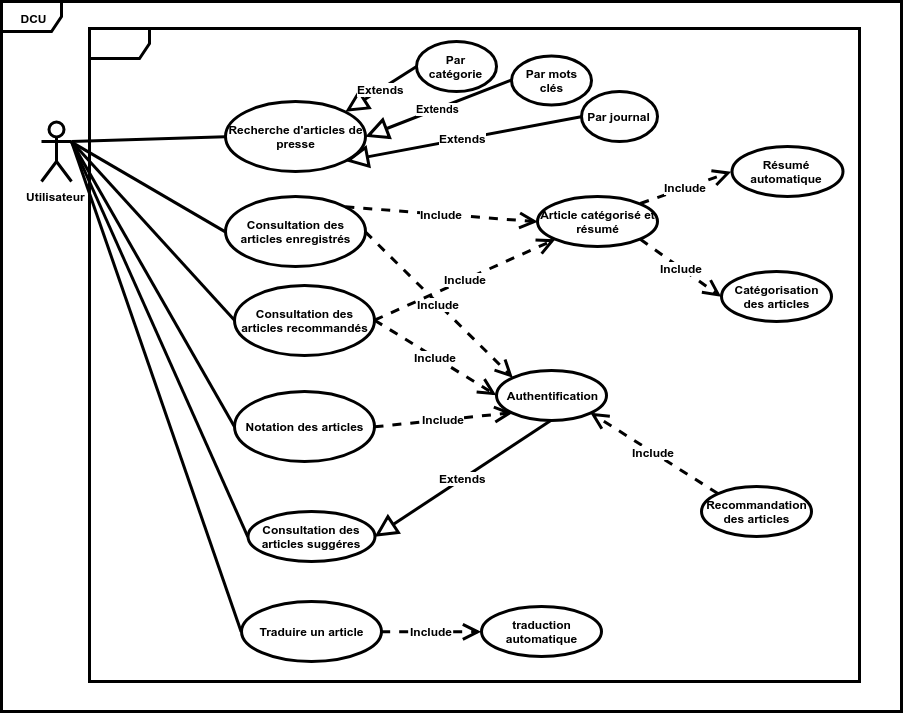
\includegraphics[height=400pt,width=350pt]{img/chapter3/diagcasdutilisation.png}
    \caption{Diagramme présentant les cas d'utilisations}
\end{figure}

\subsection{Diagramme de séquence}
Le diagramme de séquence est un diagramme UML qui fait partie des diagrammes comportementaux (dynamiques) dont L'objectif est de représenter les interactions entre les objets et les acteurs ou bien entre objets uniquement  en indiquant la chronologie des échanges. Cette représentation peut se réaliser en considérant les différents scénarios associés.\cite{UML}


\subsubsection{Diagrammes de séquence de "Feedny"}

\begin{figure}[H]
    \centering
    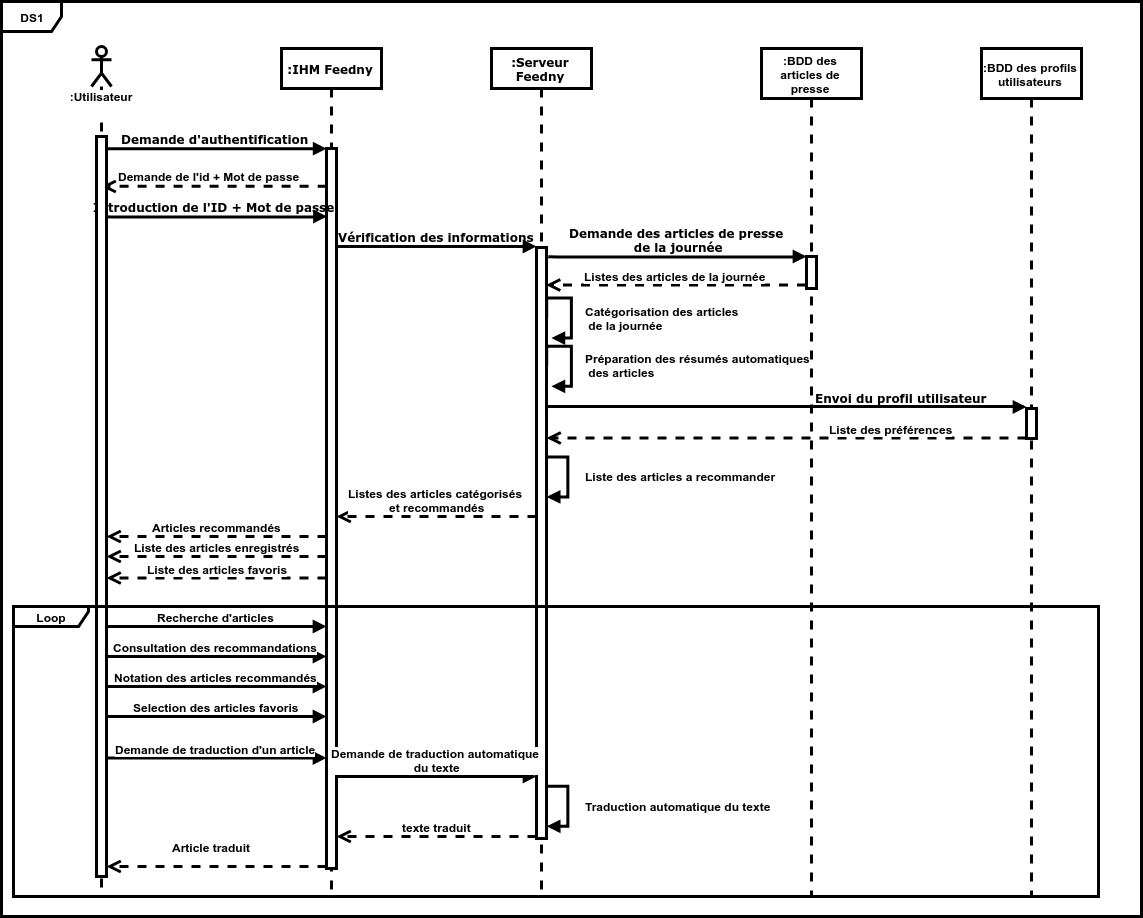
\includegraphics[height=500pt,width=425pt]{img/chapter3/diagseqperso.png}
    \caption{Diagramme de séquence dans le cas personnalisé}
\end{figure}


\begin{figure}[H]
    \centering
    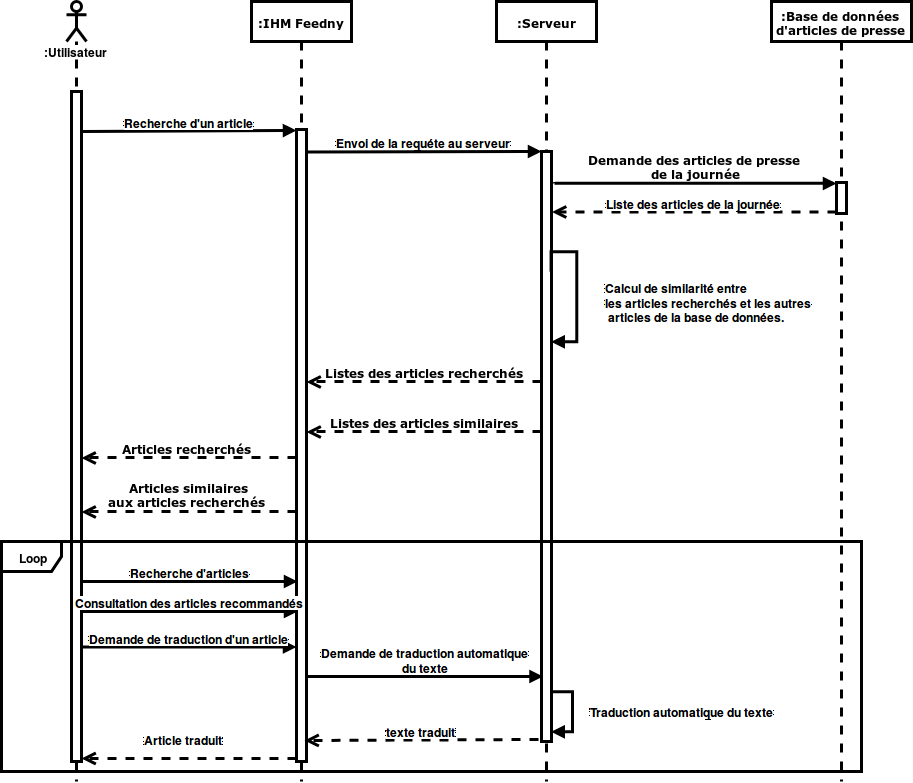
\includegraphics[height=500pt,width=425pt]{img/chapter3/diagseqnonperso.png}
    \caption{Diagramme de séquence dans le cas non personnalisé}
\end{figure}



%%%%%%%%%%%%%%%%%%%%%%%%%%%%%%%%%%%%%%%%%%%%%% Mesures d'evaluation %%%%%%%%%%%%%%%%%%%%%%%%%%%%%%%%%%%%%%%%%%%%%%%%%

\section{Mesures d'évaluation du système}

\subsection{Métriques d'évaluations du module de résumé automatique}

\subsubsection{Métrique d'évaluation : ROUGE\label{metrique-eval}}
ROUGE est l'acronyme de "Recall-Oriented Understudy for Gisting Evaluation". Il s'agit essentiellement d'un ensemble de métriques permettant d'évaluer le résumé automatique de textes ainsi que la traduction automatique. Il fonctionne en comparant un résumé produit automatiquement ou une traduction à un ensemble de résumés de référence (généralement produits par des humains). \cite{rouge0}

\subsubsection{Types des métriques de ROUGE\label{type-rouge}}
\begin{itemize}
    \item{ROUGE-1, 2, 3 et 4 : font référence au chevauchement des uni-grammes, bi-grammes, tri-grammes et quadri-grammes, respectivement, entre le système et les résumés de référence \cite{rouge1}.}\\
    \item{ROUGE-L, W : basés sur la plus longue sous-séquence commune (LCS) \cite{rouge2}.}\\
    \item{ROUGE-S : basé sur les cooccurrences des paires de mots dans l'ordre des phrases \cite{rouge2}.}\\
    \item{ROUGE-SU : en plus des paires de mots, il utilise aussi la cooccurrence du mot unique toujours dans l'ordre des phrases.}
\end{itemize}

Les métriques citées dans la \autoref{type-rouge}, utilisent comme mesures le rappel, la précision et la f-mesure :  
\begin{itemize}
    
    \item {Le rappel dans le cas de ROUGE, donne une information sur le nombre de mots du résumé de référence ont été capturés par le résumé de notre généré par le système.\\ 
        Exemple: si le rappel est égal a 40\%, cela signifie que 40\% des n-grammes du résumé de référence sont également présents dans le résumé généré par le système.}\\
    \item {La précision quant à elle, mesure la partie du résumé du système qui est pertinente ou nécessaire.\\ 
        Exemple : si la précision est égale a 40\%, cela signifie que 40\% des n-grammes du résumé généré par le système sont également présents dans le résumé de référence.}
    \item {La f-mesure dépend de la précision et le rappel et est calculé comme suit :\\
                        \[ F-mesure = \frac{2 * (Precision * Rappel)} {(Precision + Rappel)} \]}

\end{itemize}

\subsection{Métriques d'évaluations du module de catégorisation}
\begin{itemize}
    \item{\textbf{Accuracy :} }c'est une mesure qui évalue l'efficacité globale de l'algorithme par rapport au données de test.
    \[ Accuracy = \frac{tp+tn} {tp+fp+tn+fn} \]
    \item{\textbf{Précision :} }elle évalue le pouvoir prédictif du modèle en mesurant la capacité du modèle à prédire que des classes correctes.
    \[ Precision = \frac{tp} {tp+fp} \]
    \item{\textbf{Rappel :} }la capacité d’un modèle à prédire toutes les classes correctes de l'ensemble de test.
    \[ Rappel = \frac{tp} {tp+fn} \]
    \item{\textbf{F-mesure :} }une mesure composite qui profite aux algorithmes avec une sensibilité plus élevée et des algorithmes de défis avec spécificité plus élevée.!!!
    \[ F-mesure = \frac{2 * (Precision * Rappel)} {(Precision + Rappel)} \]
\end{itemize}
Avec :
\begin{itemize}
    \item{\textbf{TP }True Positive (vrais positifs) :} nombre d'individus bien prédits dans la classe à juste titre.
    \item{\textbf{FP }False Positive (faux positifs) :} nombre d'individus prédits d'une classe alors qu'ils ne devraient pas en faire parti.
    \item{\textbf{FN }False Negative (faux négatifs) :} nombre d'individus prédits comme étant de la classe alors qu'il ne le sont pas en vrai.
    \item{\textbf{TN }True Negative (vrais négatifs) :} nombre d'individus prédits comme n'étant pas dans la classe à juste titre.
\end{itemize}